\documentclass[12pt,a4paper]{report}

\usepackage{etoolbox}% http://ctan.org/pkg/etoolbox

\usepackage{lmodern} % add the missing package for font shapes
\usepackage[]{qcircuit}

\usepackage{amsmath}
\usepackage{amssymb}
\usepackage{amsfonts}

\setcounter{secnumdepth}{3}
\renewcommand\familydefault{\sfdefault} % sans serif

\usepackage[margin=2.54cm]{geometry}	% dimensiuni pagină și margini
\usepackage{graphicx} % support the \includegraphics command and options

% formatting sections and subsections
\usepackage{textcase}
\usepackage[titletoc, title]{appendix}
\usepackage{titlesec}
\titleformat{\chapter}{\large\bfseries\MakeUppercase}{\thechapter}{3ex}{}[\vspace*{-1.5cm}]
\titleformat*{\section}{\large\bfseries}
\titleformat*{\subsection}{\large\bfseries}
\titleformat*{\subsubsection}{\large\bfseries}

\usepackage{chngcntr}
\counterwithout{figure}{chapter} % no chapter number in figure labels
\counterwithout{table}{chapter} % no chapter number in table labels
\counterwithout{equation}{chapter} % no chapter number in equation labels

\usepackage{booktabs} % for much better looking tables
\usepackage{url} % Useful for inserting web links nicely
\usepackage[bookmarks,unicode,hidelinks]{hyperref}

\usepackage{array} % for better arrays (eg matrices) in maths
\usepackage{paralist} % very flexible & customisable lists (eg. enumerate/itemize, etc.)
\usepackage{verbatim} % adds environment for commenting out blocks of text & for better verbatim
\usepackage{subfig} % make it possible to include more than one captioned figure/table in a single float
\usepackage{enumitem}
\setlist{noitemsep}

%%% HEADERS & FOOTERS
\usepackage{fancyhdr}
\pagestyle{empty}
\renewcommand{\headrulewidth}{0pt}
\renewcommand{\footrulewidth}{0pt}
\lhead{}\chead{}\rhead{}
\lfoot{}\cfoot{\thepage}\rfoot{}



\newcommand{\HeaderLineSpace}{-0.25cm}
\newcommand{\UniTextEN}{POLYTECHNIC UNIVERSITY OF BUCHAREST \\[\HeaderLineSpace]
FACULTY OF AUTOMATIC CONTROL AND COMPUTERS \\[\HeaderLineSpace]
COMPUTER SCIENCE AND ENGINEERING DEPARTMENT\\}
\newcommand{\DiplomaEN}{BACHELOR THESIS}
\newcommand{\AdvisorEN}{Thesis advisor:}
\newcommand{\BucEN}{BUCHAREST}

\newcommand{\frontPage}[6]{
\begin{titlepage}
\begin{center}
{\Large #1}  % header (university, faculty, department)
\vspace{50pt}
\begin{tabular}{p{4.15cm}p{6cm}p{4.15cm}}
\vspace{-1pt}

\includegraphics[scale=0.12]{pics/upb.png} &
\vspace{-6.5pt}
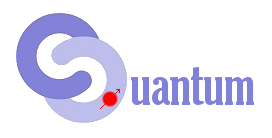
\includegraphics[scale=0.6]{pics/LogoIQC.png} &
\vspace{-2pt}

\includegraphics[scale=0.22]{pics/cs.png}
\end{tabular}

\vspace{68.5pt}
{\Huge #2}\\                           % diploma project text
\vspace{40pt}
{\Large #3}\\ \vspace{25pt}  % project title
{\Large #4}\\                          % project subtitle
\vspace{40pt}
{\LARGE \Name}\\                   % student name
\end{center}
\vspace{60pt}
\begin{tabular*}{\textwidth}{@{\extracolsep{\fill}}p{6cm}r}
&{\large\textbf{#5}}\vspace{10pt}\\      % scientific advisor
&{\large \Advisor}                                    % advisor name
\end{tabular*}
\vspace{20pt}
\begin{center}
{\large\textbf{#6}}\\                                % bucharest
\vspace{0pt}
{\normalsize \Year}
\end{center}
\end{titlepage}
}

\newcommand{\frontPageEN}{\frontPage{\UniTextEN}{\DiplomaEN}{\ProjectTitleEN}{\ProjectSubtitleEN}{\AdvisorEN}{\BucEN}}

\linespread{1.1}
\setlength\parindent{0pt}
\setlength\parskip{.23cm}

%% Abstract macro
\newcommand{\AbstractPage}{
\begin{titlepage}
\vspace*{-70pt}
{\large \textbf{ABSTRACT}}\vspace{10pt}\\
\AbstractEN \vfill
\end{titlepage}
}

%% Thank you macro
\newcommand{\ThanksPage}{
\begin{titlepage}
\vspace*{-70pt}
{\large \textbf{ACKNOWLEDGEMENTS}}\vspace{10pt}\\
\Thanks \vfill
\end{titlepage}
}



%%%%%%%%%%%%%%%%%%%%%%%%%%%%%%%%%%%%%%%%%%%%%%%%%%   
%%
%%          End of template definitions
%%   
%%%%%%%%%%%%%%%%%%%%%%%%%%%%%%%%%%%%%%%%%%%%%%%%%%


%%% Puteți elimina aceste linii din lucrare, servesc numai pentru template.
\newcommand{\worktype}[1]{[\textit{#1}] }
\newcommand{\dezvoltare}{\worktype{Dezvoltare de produs}}
\newcommand{\cercetare}{\worktype{Cercetare}}
\newcommand{\ambele}{\worktype{Ambele}}
%%%


%%
%%   Campurile de mai jos trebuie modificate de autor. Modificati doar continutul, nu si numele fiecarei definitii
%%
\newcommand{\ProjectTitleEN}{A comprehensive study on Integrating Quantum Physics in Deep Learning Networks for Optimizations in Computer Vision and Natural Language Processing Fields}
\newcommand{\ProjectSubtitleEN}{QRKT-GAN: Neural Ordinary Differential Equation-Inspired Generative Adversarial Network with Numerical Runge-Kutta Methods for Quantum Visual Transformer-Based Generator and Discriminator}
\newcommand{\Name}{Cătălin-Alexandru Rîpanu}
\newcommand{\Advisor}{Șl. dr. ing. Dumitru-Clementin Cercel}
\newcommand{\Year}{2024}

% Setări document
\title{Diploma Project}
\author{\Name}
\date{\Year}

%%
%%   Campurile aferente rezumatului
%%

\newcommand{\AbstractEN}{Deep Learning models, such as Generative Adversarial Networks (GANs)~\cite{goodfellow2014generative} and Visual Transformers (ViTs)~\cite{vaswani2017attention, dosovitskiy2020}, have demonstrated remarkable results across various domains in Machine Learning and Artificial Intelligence, including Object Classification, Image Segmentation, Sentiment Analysis, and Synthetic Data Generation. These neural networks are pivotal in advancing systems that require high precision and a deep understanding of complex data across a variety of tasks in both Natural Language Processing (NLP) and Computer Vision (CV).

However, the effectiveness of Deep Learning models comes with significant challenges: they require an extensive~\cite{chen2014big} number of parameters to learn and extract meaningful features from real-world data. Additionally, these models need vast amounts of information to achieve desired performance levels. Obtaining such large sets can be difficult as real-world data is often not publicly available and can be challenging to collect and curate. This results in substantial computational resource requirements for both training and hyperparameter optimization, often achieved through exhaustive techniques such as grid search~\cite{liashchynskyi2019grid}.

To address these challenges, this thesis proposes a novel hybrid Generative Adversarial Network architecture that employs Quantum Visual Transformers (QViTs)~\cite{di2022dawn} as both the Generator and Discriminator. Visual Transformers~\cite{vaswani2017attention, dosovitskiy2020} are selected for their superior ability to manage intricate data representations. A key innovation in this architecture is the integration of Ordinary Differential Equation (ODE)~\cite{fan2024Quantum} solvers as Encoders~\cite{hinton2011transforming}, enhancing the model capability to capture temporal dynamics and complex data structures, and improving the residual connections within the transformer architecture to mitigate the vanishing gradients problem~\cite{liu2020understanding} even more.

Moreover, this architecture incorporates Variational Quantum Circuits~\cite{cerezo2021variational} within both the Self-Attention Mechanisms~\cite{voita2019analyzing} and the Multi-Layer Perceptrons (MLPs)~\cite{popescu2009multilayer} of the Visual Transformers~\cite{vaswani2017attention, dosovitskiy2020}. By leveraging the principles of Quantum Mechanics, these Quantum circuits~\cite{benedetti2019parameterized} can perform complex algebraic operations more efficiently than classical methods, offering a significant computational advantage.

The performance of this hybrid approach is benchmarked against a purely classical neural network baseline from the literature using datasets from both CV and NLP areas. Specifically, the Quantum ODE configurations are tested on CIFAR-10~\cite{Krizhevsky09learningmultiple}, CIFAR-100~\cite{Krizhevsky09learningmultiple}, MNIST~\cite{lecun2010mnist}, IMDb Reviews~\cite{maas-EtAl:2011:ACL-HLT2011} and ILSVRC 2012~\cite{ILSVRC15}  datasets. These neural network architectures are effectively trained and tested using numerical simulations tailored to Quantum circuits~\cite{Zhang_2023}. The obtained results indicate that these hybrid approaches achieves comparable classification and generation performance to the classical baseline, while requiring fewer trainable parameters.

Furthermore, the reduced parameter count in these hybrid models opens up the possibility of running it on Noisy Intermediate-Scale (NISQ)~\cite{lau2022nisq} quantum devices for both training and inference. This feasibility is a significant breakthrough, as it implies that quantum-enhanced models can be trained and deployed on actual quantum computers, which are currently limited in terms of the number of qubits and operational fidelity~\cite{lau2022nisq}.

This thesis demonstrates the potential of integrating Quantum Computing~\cite{nielsen2001quantum}, especially Quantum Mechanics, with advanced Deep Learning architectures to create more efficient and powerful networks which can significantly reduce computational costs while maintaining high performance, paving the way for more scalable and effective AI applications~\cite{huang2021power}.}

%%
%%   Campurile aferente paginii de multumiri
%%
\newcommand{\Thanks}{
First and foremost, I would like to express my deepest gratitude to my advisor, Prof. Dumitru-Clementin Cercel, for his unwavering support and insightful guidance throughout my research journey. His expertise and encouragement have been essential in exploring the intricate intersection of Machine Learning and Quantum Mechanics, widely referred to in the literature as Quantum Machine Learning. This interdisciplinary field, though initially daunting, is at the cutting edge of technological advancement and innovation in both areas.

I am also profoundly thankful to Prof. Pantelimon-George Popescu for his advice, recommendations, and exceptional lectures on Quantum Computing. His mentorship has been instrumental in building a robust understanding of this groundbreaking paradigm, which promises new solutions to problems previously deemed insurmountable by classical methods.

Furthermore, I wish to acknowledge the significant contributions of the academic teaching assistants and collaborators encountered during my bachelor's studies. Their guidance during challenging times has been crucial to my academic development. Last but not least, I am also grateful for the computational resources provided by the Computer Science and Engineering Department, which were essential for the design and implementation of this project.

In addition, I extend my appreciation to my friends for their continuous support, ideas, and advice, especially during moments when inspiration was scarce. Lastly, my heartfelt thanks go to my parents for their enduring sacrifices and unwavering support throughout this journey into the unknown. Their belief in me has been a constant source of motivation.
}

\makeatletter
\def\@makechapterhead#1{%
  \vspace*{-55\p@}%
  {\parindent \z@ \raggedright \normalfont
  \ifnum \c@secnumdepth >\m@ne
  \Large\bfseries \thechapter\space% Adjust the size as needed
  \fi
  \interlinepenalty\@M
  \Large \bfseries #1\par\nobreak
  \vskip 12\p@
  }}
  
\makeatother

\begin{document}

\setcounter{page}{1}
\frontPageEN


\setcounter{page}{2}
\ThanksPage \pagestyle{fancy}

\AbstractPage\pagestyle{fancy}

\renewcommand{\contentsname}{\vspace{-3.45cm} CONTENTS}
\tableofcontents
% Textul licentei incepe de aici 

\chapter{Introduction}\pagestyle{fancy}

\section{Context}\vspace{-12pt}
Artificial Intelligence models, particularly Deep Learning ones, have made significant contributions to solving real-world tasks, greatly improving human lives in various fields, such as Medical Image Recognition~\cite{he2020infusing}. Despite their impressive capabilities, Deep Learning models come with substantial drawbacks regarding computational resources~\cite{chen2014big} and effort. Achieving high performance with these models necessitates learning millions to billions of parameters, also called weights or artificial neurons, which demands considerable resources and preparation time. This limitation also has negative environmental impacts due to high power consumption.

Over the years, researchers have developed numerous solutions to mitigate the problem of minimizing the number of parameters using interesting classical algorithms and techniques. These include, for example, specialized activation functions for neural layers like Rectified Linear Unit~\cite{NIPS2017_a96b65a7}, Leaky ReLU~\cite{xu2020reluplex}, Gaussian Error Linear Unit~\cite{hendrycks2016gaussian}, Softmax~\cite{liu2016large}, Sigmoid~\cite{han1995influence} and Hyperbolic Tangent~\cite{zamanlooy2013efficient}. Additionally, effective optimizers such as Adam~\cite{zhang2018improved} and Stochastic Gradient Descent~\cite{bottou2010large} have been utilized to combat this limitation, along with methods like Learning Rate Schedulers~\cite{wen2021convolutional}, Weight Decay~\cite{loshchilov2017decoupled}, and Dropout~\cite{srivastava2014dropout} to reduce also the chances of model overfitting. Over the years, various architectural designs and network combinations have emerged to address these challenges. However, the tradeoff between high computational resource consumption and performance remains a difficult issue, especially when scaling up the dimensions of available noisy real-world datasets used for training. It is unlikely\footnote{\url{https://www.theverge.com/24066646/ai-electricity-energy-watts-generative-consumption}} to be efficiently resolved in the near future using solely classical approaches.

A segment of Computer Science researchers, in collaboration with physicists, have taken a bold and innovative approach to these challenges by exploring solutions from a physical perspective, leading to the emergence of Quantum Computation and Quantum Information~\cite{nielsen2001quantum}. Leveraging the principles of Quantum Mechanics, AI research has begun to explore Deep Learning optimizations using quantum facilities, such as Variational Quantum Circuits~\cite{benedetti2019parameterized} or Quantum Algorithms~\cite{cerezo2021variational}, to develop hybrid Deep Learning models. By combining classical and quantum methodologies, new experiments can be conducted to address performance and resource demands more efficiently, thus utilizing the unique capabilities of quantum hardware. This involves training these models on it, also known as Parameterized Quantum Circuits~\cite{benedetti2019parameterized}, where the parameters are referred to as the qurons of the quantum model.

Quantum Computing leverages properties like superposition~\cite{koprinkov2023quantum} and entanglement~\cite{Horodecki_2009}, enabling the execution of complex algebraic operations that are infeasible for classical computers. Quantum Algorithms~\cite{cerezo2021variational}, such as Grover's Algorithm~\cite{shi2017coherence}, Quantum Phase Estimation~\cite{o2019quantum}, Quantum Fourier Transform~\cite{weinstein2001implementation} and Deutsch-Jozsa Quantum Parallelism~\cite{gulde2003implementation} provide exponential speedups for certain tasks. Integrating these Quantum principles with Deep Learning can significantly reduce the number of parameters and computational resources required while maintaining or even enhancing model performance. This interdisciplinary distinctive approach, also known as Quantum Machine Learning, opens up exciting possibilities for the future of AI, promising advancements that could transform how complex problems are approached and solved in ways that classical computers, with their current architecture, could never achieve.
\section{Problem}\vspace{-12pt}
Over the years, numerous algorithms, techniques, network architectures, and methodologies have been proposed in the field of Deep Learning to tackle a wide array of tasks, such as Object Classification, Synthetic Data Generation and Detection, across various domains including Natural Language Processing, Computer Vision, Domain Adaptation~\cite{farahani2020brief}, and Knowledge Distillation~\cite{hinton2015distilling}. These approaches have achieved high performance metrics like Accuracy, Area Under the Curve (AUC), Receiver Operating Characteristic (ROC), and F1 scores. The advent of High Performance Computing (HPC) facilities, particularly classical parallelism, has enabled Deep Learning models to process billions of examples from noisy real-world datasets effectively, thus yielding impressive results.

Despite these advancements, a significant drawback persists: the enormous number of neurons and the corresponding computational resources required by these models. Traditional solutions in classical Deep Learning, such as Cross Validation~\cite{berrar2019cross}, Hyperparameter Tuning techniques like Grid Search~\cite{liashchynskyi2019grid} or Random Search~\cite{liashchynskyi2019grid}, Keras Tuner~\cite{pon2021hyperparameter}, and Layer Augmentation until model performance plateaus or overfits, are commonly employed. To mitigate overfitting, regularization techniques such as Ridge~\cite{ogutu2012genomic}, Lasso~\cite{ogutu2012genomic}, Elastic-Net~\cite{ogutu2012genomic} or Dropout~\cite{srivastava2014dropout} can be applied. However, these methods often involve exhaustive hyperparameter searches, which are extremely time-consuming, especially when dealing with validation sets comprising billions of data points for complex tasks. Furthermore, group sparsity regularizers can be applied to network parameters, where each group acts on a single neuron, thus reducing the number of parameters by up to 80\% while maintaining or even enhancing the network accuracy score~\cite{alvarez2018learning}.

Another method employed to address these challenges is Transfer Learning~\cite{weiss2016survey}, which involves finding and loading a pretrained model as a starting point and then fine-tuning it on a specific dataset. This approach can help achieve good performance with less effort on architecture design and expedite the training process. However, the availability of suitable pretrained models is limited, and fine-tuning may yield only decent, if not disappointing, results, due to differences in the data distributions between the pretraining and fine-tuning datasets.

The primary challenge lies in balancing time, memory and power consumption on classical systems to make robust and valid neural architectural choices. Furthermore, reducing the number of neurons too drastically is not a solution as it can lead to underfitting and degraded performance, making it difficult to solve complex and challenging tasks efficiently. The iterative process of tuning hyperparameters and optimizing model architectures is computationally intensive and often results in a significant trade-off between resource consumption and model performance~\cite{liashchynskyi2019grid}.

Moreover, the reliance on vast amounts of training data for achieving desired performance further exacerbates these issues. Real-world datasets are often difficult to obtain and may not be publicly available, which complicates the development and fine-tuning of effective Deep Learning models. The extensive time and computational costs associated with hyperparameter optimization and model training present significant obstacles to advancing AI capabilities while maintaining efficiency and sustainability. This trade-off between computational resource consumption and performance remains a persistent and challenging problem in the field of Deep Learning, highlighting the need for innovative solutions that can overcome these limitations.

\section{Objective}\vspace{-12pt}
In the current landscape of Deep Learning research, there is an ongoing investigation into whether integrating models into a purely quantum environment can significantly reduce power consumption and the number of trainable parameters without sacrificing performance. This exploration leverages techniques such as the Ansatz~\cite{hadfield2019Quantum} and Variational Quantum Circuits~\cite{cerezo2021variational}. As classical supercomputers advance to handle increasingly complex deep models, their power consumption grows almost exponentially. In contrast, quantum machines exhibit an exponential increase in computational power while maintaining a linear increase in power consumption. This intriguing characteristic makes a strong case for Quantum Computing: with the advent of fault-tolerant quantum computers, qubits could serve as highly efficient artificial neurons in neural networks. Quantum-inspired techniques could enable networks to operate with a vast number of neurons per layer at minimal energy cost, dramatically reducing overall energy consumption\footnote{\url{https://www.eetimes.eu/how-Quantum-Computing-can-help-make-ai-greener}}.

Building on the challenges outlined in the above section, the primary goal of this thesis is to explore Deep Learning models, both pure Quantum and hybrid, that leverage neural ODE-based architectures~\cite{zhong2022neural} inspired by non-trivial Variational Quantum Circuits~\cite{cerezo2021variational} within the context of Visual Transformers~\cite{vaswani2017attention, dosovitskiy2020} and their complex Encoders~\cite{hinton2011transforming} and Decoders~\cite{breuckmann2018scalable}. The most important objective is to minimize the number of parameters used by deep network layers utilizing the idea~\cite{Comajoan_Cara_2024} of replacing classical linear projection layers in Multi-Head Attention~\cite{voita2019analyzing} subroutines and Multi-Layer Perceptrons~\cite{popescu2009multilayer} with Quantum Circuits~\cite{benedetti2019parameterized}. Additionally, low truncation error Neural Ordinary Differential Equation~\cite{zhong2022neural}\cite{li2022ode} techniques will be employed to further optimize Transformer Layers, namely Runge-Kutta Methods~\cite{butcher1996history} of 1st, 2nd, 3rd, and 4th order. An analysis of Runge-Kutta 4th order method optimization which is not theoretically grounded in standard RK methods, but in terms of training, will also be included~\cite{li2022ode}.

To better understand the rationale and motivation behind the proposed Deep Learning model in this paper, it is necessary to compare these Quantum ODE-based Transformers configurations  with their classical counterparts using the datasets mentioned in Abstract. The network utilizing the optimized Runge-Kutta 4th order method will be leveraged within the context of Vision Transformers (ViTs)~\cite{vaswani2017attention, dosovitskiy2020} and integrated into a Generative Adversarial Network (GAN)~\cite{goodfellow2014generative} architecture. In this configuration, both the Generator and Discriminator will be Quantum Visual Transformers (QViTs)\footnote{\url{https://openreview.net/pdf?id=p7xPXoKB0H}}, incorporating the optimized Neural ODE solver to generate realistic and informative synthetic data without being limited to specific types of distributions. This will be achieved using techniques such as Data Augmentation~\cite{zhao2020diffaugment} and Image Recognition at Scale~\cite{dosovitskiy2020} in the context of ViTs~\cite{vaswani2017attention}.

The final proposed architecture in this thesis, named QRKT-GAN, will be tested on a real-world consistent dataset, namely CIFAR-10~\cite{Krizhevsky09learningmultiple}, and compared using the same data with a renowned classical counterpart, TransGAN~\cite{jiang2021transgan}, which is a strong architecture built entirely free of Convolutions~\cite{cordonnier2020relationship}. This comparative analysis will provide another argument for the possible advantages of integrating Quantum Computing~\cite{nielsen2001quantum} with advanced Deep Learning neural networks under the right context.
\section{Paper Structure}\vspace{-12pt}
The next chapter delves into the most relevant and important classical and Variational Quantum Algorithms~\cite{cerezo2021variational} and techniques developed over the years to leverage both Quantum and hybrid logic in Deep Learning for model optimization. This chapter will illustrate how these both hybrid and pure Quantum Neural Networks (QNNs)~\cite{breuckmann2018scalable} are designed to be compatible with Noisy Intermediate-Scale (NISQ)~\cite{lau2022nisq} devices provided by specialized vendors such as IBM~\cite{Santos_2016}, Google~\cite{kalai2023googles}, Microsoft~\cite{Mykhailova_2023}, and Amazon~\cite{Reyes_2021}. It will explore the advancements that make it possible to run complex Deep Learning models on quantum computers, highlighting the interplay between Quantum Computing~\cite{nielsen2001quantum} and Deep Learning for neural depth decreasing while not losing too much performance.

Section three will discuss the foundational concepts of Machine Learning, Deep Learning and Ordinary Differential Equations. It will also provide a comprehensive overview of Quantum Computation and Quantum Information~\cite{nielsen2001quantum}, and will also introduce the emerging field of Quantum Machine Learning~\cite{dunjko2018machine}. This section aims to explain how quantum principles can enhance the capabilities of Deep Learning solutions in addressing high-demanding tasks, some of which are classified as NP-Hard~\cite{chatterjee2024solving} or NP-Complete~\cite{furer2008solving}. By understanding these fundamentals, the reader will gain insight into the potential synergies between Classical and Quantum Computing~\cite{nielsen2001quantum}, which together can form a duality in the world of Artificial Intelligence.

Section four will present an in-depth analysis of the proposed Ordinary Differential Equation-based Quantum Neural Networks (QNNs)~\cite{abbas2021power, li2022ode} configurations. This includes their motivation, underlying concepts, mathematical and quantum frameworks, physical limitations, and future potential within their problem domain environment. The chapter will also discuss in-detail the new ODE-based GAN architecture in detail, QRKT-GAN, explaining how it incorporates the traversed knowledge to minimize the solution of the optimization problem outlined in Context section, while maintaining acceptable performance in Synthetic Image Generation.

The fifth chapter will detail the methodologies adopted for conducting the experiments. This includes a comprehensive description of the datasets used, their internal characteristics, and the reasons for their selection. It will compare various Quantum ODE-based~\cite{fan2024Quantum} configurations with their classical ODE-based networks~\cite{zhong2022neural} counterparts to fully understand the benefits and limitations of quantum-enhanced models. Additionally, the chapter will provide a detailed comparison between the proposed QRKT-GAN model and its classical baseline, TransGAN~\cite{jiang2021transgan}, using the CIFAR-10~\cite{Krizhevsky09learningmultiple} dataset. This analysis will highlight the benefits and challenges of integrating Quantum Computing into Deep Learning, presenting it as a viable alternative solution for very specific optimization problems.

The final chapter will summarize the main ideas presented in the thesis, highlighting the relevance of the results and drawing key conclusions. It will also propose future work and outline potential directions for further research in the field of Quantum Deep Learning models, focusing on power consumption, computational resources and performance optimization. This chapter will emphasize the importance of continued exploration in combining Quantum Computing with Machine Learning~\cite{dunjko2018machine} to achieve more efficient and powerful neural solutions.

\chapter{Related Work}\vspace{-12pt}
The relentless demand for improving human lives continues unabated, with increasingly complex and data-intensive needs emerging. This necessitates the development of sophisticated models capable of delivering accurate and reliable results. However, the complexity and depth of these models often result in significantly high computational resource consumption, which has environmental implications due to the energy required for such intensive processing.

Over the years, numerous classical, quantum, and hybrid methods have been proposed to address the optimization problem of minimizing model depth without significantly sacrificing performance. One notable approach is real-time learning of the number of neurons in deep networks using structured sparsity during training, which dynamically adjusts the network structure to optimize performance without excessive resource use~\cite{alvarez2018learning}. Another method involves crafting specialized architectures that maintain a constant computational budget while slightly increasing depth to improve performance. This is achieved by dimensionality reduction before applying expensive Convolutions~\cite{wen2021convolutional} with larger patch sizes~\cite{Szegedy_2015_CVPR}. Unfortunately, Convolutions~\cite{wen2021convolutional} have been shown~\cite{cordonnier2020relationship} to be less effective in capturing global feature interactions, as they primarily focus on local patterns in data processing. In contrast, the Self-Attention mechanism~\cite{voita2019analyzing} utilized in Transformers~\cite{vaswani2017attention} excels at capturing these global interactions.

In addition, some techniques focus on minimizing weights during training by splitting network weights into sets or hierarchies of multiple groups, each using disjoint sets of features. This allows parallelization, even in an embarrassingly manner, as each subnetwork operates independently, enhancing computational efficiency~\cite{pmlr-v70-kim17b}. Alternatively, population-based heuristic algorithms, such as Particle Swarm Optimization (PSO), have shown promise in optimally determining the number of parameters without exhaustive searches like grid search~\cite{liashchynskyi2019grid}, and thus saves valuable computational resources during the tuning process of these Deep Learning models~\cite{7986470}. Another approach involves reducing model parameters in deep neural networks via product-of-sums matrix decompositions, which decompose linear operators as a product of sums of simpler linear operators~\cite{wu2018prodsumnet}. For Deep Convolutional Neural Network~\cite{wen2021convolutional} models, kernel-sharing between multiple convolutional layers can also be applied~\cite{azadbakht2022drastically}. Kernel-sharing is possible only between layers having the same kernel size, input, and output channels.

Despite their advantages, these classical methods have inherent drawbacks. Designing neural architectures from scratch to meet specific requirements is challenging and time-consuming. Moreover, methods like Particle Swarm Optimization~\cite{7986470} require optimization of additional parameters, such as activation functions~\cite{han1995influence, NIPS2017_a96b65a7, xu2020reluplex} and the number of epochs, to be truly effective. Quantum Neural Networks (QNNs)~\cite{abbas2021power} and Quantum Algorithms~\cite{cerezo2021variational} offer new avenues for addressing these limitations, providing potential solutions for power-efficient Deep Learning. Various Quantum frameworks, technologies, GPU-based numerical simulators, and access to real hardware have been developed to facilitate the implementation of quantum phenomena in Machine Learning.

However, the quantum approach shares a common challenge with classical methods: the need for specific adaptations for each type of Deep Learning model.
In the classical domain, the entire architectural framework must be meticulously analyzed to prevent performance degradation. In quantum domain, constructing valid Variational Quantum Circuits (VQCs)~\cite{benedetti2019parameterized} and Algorithms~\cite{cerezo2021variational} that efficiently mimic classical functions is crucial to avoid the same pitfalls.
\chapter{Background}\vspace{-12pt}
This chapter will delve into the main and most important advancements in Machine Learning, presenting key concepts as they appeared in the literature. It will discuss the motivation and necessity of Deep Learning, a fundamental subdomain of Machine Learning, to fully understand the creation and utilization of neural networks. This will include an exploration of why Generative Adversarial Networks (GANs)~\cite{goodfellow2014generative} and Visual Transformers~\cite{vaswani2017attention, dosovitskiy2020} were developed, along with a detailed examination of their architectural specificities and functions.

Furthermore, the chapter will provide an overview of the techniques used to identify optimal hyperparameters, which are crucial for further neural model optimization. This will cover various approaches to fine-tuning Deep Learning models to enhance their performance.

A significant portion will be dedicated to Ordinary Differential Equations (ODEs) and their most popular numerical solvers, highlighting the foundational aspects of the Runge-Kutta methods~\cite{butcher1996history}. It will explain how to interpret Transformer layers from an ODE perspective~\cite{li2022ode}, providing a mathematical framework for understanding these non-trivial neural network structures.

The chapter will also present a concise summary of Quantum Computing~\cite{nielsen2001quantum}, establishing the prerequisites for understanding Quantum Machine Learning~\cite{dunjko2018machine}. This section will articulate the motivation behind integrating Runge-Kutta ODE methods~\cite{butcher1996history, fan2024Quantum} into Quantum Computing~\cite{nielsen2001quantum}. By exploring Quantum Circuits~\cite{benedetti2019parameterized} and Quantum Gates~\cite{barenco1995elementary}, Variational Quantum Algorithms~\cite{cerezo2021variational}, and Variational Quantum Circuits~\cite{benedetti2019parameterized}, the chapter will illustrate their motivation and application in the context of Quantum Transformers~\cite{Comajoan_Cara_2024}.

By comprehensively covering these topics, the chapter aims to equip readers with a deep understanding of the theoretical and practical foundations necessary for advancing in the field of Quantum Machine Learning~\cite{dunjko2018machine}, particularly through the integration of ODE methods~\cite{zhong2022neural} in quantum frameworks~\cite{Zhang_2023}.

\section{Machine Learning}\vspace{-12pt}
Machine Learning is the process of enabling computers to learn from data and make decisions without being explicitly programmed to do so. The essential aspect of Machine Learning is training models on data before they can autonomously make decisions. Thus, data is fundamental to Machine Learning algorithms. Without data, Machine Learning cannot function, as models rely entirely on the information provided to make future predictions. The data used must accurately reflect real-world scenarios because Machine Learning models depend on this data to learn and generate accurate predictions for new, unseen data~\cite{machinelearning}.

In practice, Machine Learning involves extensive mathematical operations such as matrix multiplication, feature scaling, and normalization. Consequently, the data fed into Machine Learning algorithms must be represented as numerical vectors or numbers, as opposed to text or other non-numerical forms that machines cannot directly interpret.

For instance, textual data and alphabets are not directly understandable by machines; hence, they must be converted into numerical form before being processed by Machine Learning models. Techniques such as one-hot encoding, word embeddings, or other numerical transformation methods are used to convert text into a machine-readable format, enabling models to learn from and predict based on the data provided~\cite{machinelearning}.

Machine Learning algorithms, along with neural networks, have been proposed for many decades. However, during the early days, the lack of sufficient data and limited computational power hindered their practical application. Today, the scenario has drastically changed. Companies generate vast amounts of data, and computational resources have become extraordinarily powerful and accessible. Services like Google Cloud and Amazon Web Services (AWS) provide scalable computational power, allowing users to run complex Machine Learning algorithms without the need for setting up their own hardware infrastructure. This has led to an exponential growth in the demand for Machine Learning and Deep Learning applications~\cite{machinelearning}.

Understanding Machine Learning and Deep Learning is crucial in this data-rich environment. The ability to harness data through these technologies enables companies to make informed predictions, optimize processes, and drive innovation. The more effectively Machine Learning models are trained and utilized, the greater the value they can bring to an organization, ultimately contributing to increased profitability and competitive advantage.

Types of Machine Learning~\cite{machinelearning}:
\begin{itemize}
  \item \textbf{Supervised learning} involves training a Machine Learning model on a labeled dataset, where the output labels are known. The model learns to map inputs to outputs based on this labeled data. During training, the model predictions are compared with the actual labels to evaluate its performance and adjust its parameters accordingly. This iterative process continues until the model achieves satisfactory accuracy. An example of supervised learning is predicting house prices. Given a dataset with features like square footage, number of bedrooms, and location, along with corresponding house prices, the model learns to predict the price of a house based on these features. By comparing its predictions with the actual prices, the model improves over time.
  \item \textbf{In unsupervised learning}, the model is trained on data without labeled outputs. The goal is for the model to identify patterns, structures, or relationships within the data. One common application of unsupervised learning is customer segmentation, where customers are grouped based on their behavior, such as purchase history or browsing patterns, without pre-defined labels. This helps businesses tailor marketing strategies to different customer segments.
  \item \textbf{Semi-supervised learning} combines elements of both supervised and unsupervised learning. It uses a small amount of labeled data along with a larger amount of unlabeled data. The model is initially trained on the labeled data, and then it generalizes its learning to the unlabeled data. This approach is useful when obtaining labeled data is expensive or time-consuming. An example of semi-supervised learning is text document classification. A model is first trained on a subset of documents with known categories. Then, it is used to classify the remaining documents, which do not have predefined labels, based on the patterns it has learned.
\end{itemize}

\section{Gradient Descent}\vspace{-12pt}
Gradient Descent (GD) is a foundational first-order optimization algorithm widely used in Machine Learning (ML) and Deep Learning (DL) for minimizing cost or loss functions. This iterative method works by iteratively adjusting the parameters of a model to find the local minimum or maximum of a given function, thereby improving the model accuracy. For instance, in linear regression, Gradient Descent helps minimize the difference between predicted and actual values by updating the weights and biases. Its significance and simplicity make it a fundamental topic in nearly all introductory Machine Learning courses, as it provides a clear understanding of how models learn and improve from data~\cite{gradientdescent}.

The Gradient Descent algorithm is not universally applicable to all functions. For it to work effectively, the function must meet two specific criteria: it must be differentiable and convex.

Mathematically:
\begin{itemize}
  \item A function is differentiable if it has a derivative at each point in its domain. This means the function must be smooth and continuous without any sharp corners or discontinuities. Differentiability is crucial because Gradient Descent relies on the gradient (the derivative) to determine the direction and magnitude of the steps to take towards the minimum or maximum. If the function is not differentiable, the algorithm cannot compute the gradient accurately, leading to unreliable optimization results.
        \begin{figure}[th]
          \centering
          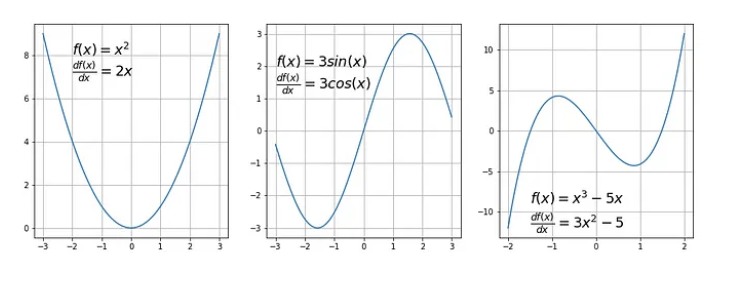
\includegraphics[scale=0.637]{./pics/diff_func.png}
          \caption[Examples of differentiable functions]{Examples of differentiable functions. Image from~\cite{gradientdescent}.}
          \label{fig:pic1}
        \end{figure}
        \begin{figure}[th]
          \centering
          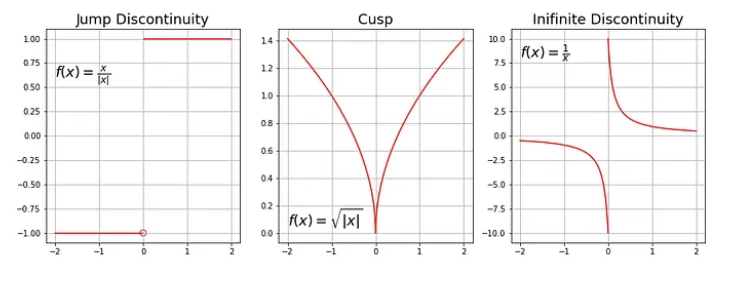
\includegraphics[scale=0.637]{./pics/undiff_func.png}
          \caption[Examples of non-differentiable functions]{Examples of non-differentiable functions~\cite{gradientdescent}.}
          \label{fig:pic2}
        \end{figure}
  \item A function is convex if the line segment between any two points on the function graph lies above or on the graph. Formally, a function \( f(x) \) is said to be convex if for all \( x_1 \) and \( x_2 \) in its domain, and for all \( \lambda \) in the interval \([0, 1]\), the following inequality holds:
        \begin{equation}
          f(\lambda x_1 + (1 - \lambda) x_2) \leq \lambda f(x_1) + (1 - \lambda) f(x_2)
        \end{equation}
        Convexity ensures that any local minimum is also a global minimum, making it easier for Gradient Descent to find the optimal solution.
        \begin{figure}[th]
          \centering
          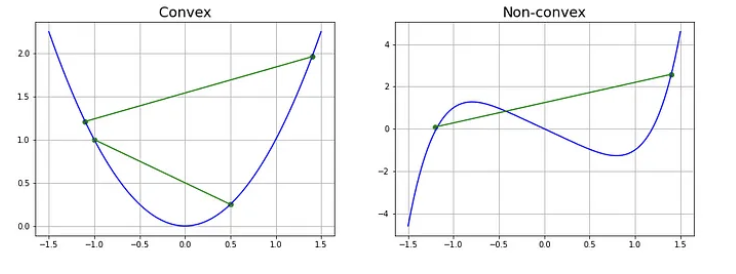
\includegraphics[scale=0.637]{./pics/conv_unconv_func.png}
          \caption[Examples of non-differentiable functions]{Examples of convex and non-convex functions~\cite{gradientdescent}.}
          \label{fig:pic3}
        \end{figure}
\end{itemize}

Gradient Descent is an optimization algorithm used to minimize a function by iteratively moving towards the steepest descent direction. At each step, it calculates the gradient of the function at the current point, scales it by a learning rate, and updates the position by moving in the opposite direction of the gradient. This process ensures that the algorithm moves towards the function minimum. The update rule can be expressed as:

\begin{equation}
  \mathbf{a}_{n} = \mathbf{a}_{n-1} - \eta \nabla f(\mathbf{a}_{n-1})
\end{equation}

where:
\begin{itemize}
  \item $\mathbf{a}_{n-1}$ is the current position.
  \item $\eta$ is the learning rate.
  \item $\nabla f(\mathbf{a}_{n-1})$ is the gradient of the function at the current position.
\end{itemize}

By repeatedly applying this update rule, Gradient Descent converges to the minimum of the function. If the goal were to maximize the function, the algorithm would instead add the scaled gradient~\cite{gradientdescent}.

The learning rate, denoted as \(\eta\), is a crucial hyperparameter in gradient descent algorithms that determines the step size at each iteration while moving toward a minimum of the loss function. The choice of learning rate significantly affects the performance of the algorithm:

\begin{itemize}
  \item \textbf{Small Learning Rate}: If the learning rate is too small, the convergence process will be slow, potentially requiring many iterations to reach the optimal point. In some cases, the algorithm may even hit the maximum number of iterations before converging.
  \item \textbf{Large Learning Rate}: If the learning rate is too large, the algorithm might not converge to the optimal point. Instead, it could overshoot the minimum, causing the algorithm to oscillate or even diverge entirely, failing to find a satisfactory solution.
\end{itemize}

Thus, selecting an appropriate learning rate is essential for the efficient and effective training of Machine Learning models~\cite{gradientdescent}.

\subsection{AdamW Optimizer}

Adam combines the strengths of both Stochastic Gradient Descent (SGD)~\cite{bottou2012stochastic} with Momentum and Root Mean Square Propagation (RMSProp). It calculates the exponential moving averages of the gradient first and second moments. Like SGD with Momentum, it helps smooth out the updates to accelerate convergence. Similar to RMSProp, Adam uses adaptive learning rates for each parameter, allowing smaller steps for steep gradients and larger steps for flatter areas. Additionally, Adam adjusts these learning rates by considering both the mean of the first moment (the gradient) and the mean of the second moment (the squared gradient). The parameter update rule in Adam is given by~\footnote{\url{https://www.linkedin.com/pulse/understanding-adam-adamw-dsaisolutions-ileof/}}:
\begin{equation}
  \theta_{t+1} = \theta_t - \eta \frac{\hat{m}_t}{\sqrt{\hat{v}_t} + \epsilon}
\end{equation}
\begin{equation}
  m_t = \beta_1 m_{t-1} + (1 - \beta_1) \nabla_\theta f(\theta_t)
\end{equation}
\begin{equation}
  v_t = \beta_2 v_{t-1} + (1 - \beta_2) (\nabla_\theta f(\theta_t))^2
\end{equation}
where:

\begin{itemize}
  \item \(\theta\) is the parameter to be updated
  \item \(\eta\) is the initial learning rate
  \item \(\beta_1\) is a decay rate for the first moment, with a default value of 0.9
  \item \(\beta_2\) is a decay rate for the second moment, with a default value of 0.999
  \item \(\epsilon\) is a small number used to avoid division by zero
  \item \(\nabla_\theta f(\theta)\) is the gradient of the loss function \(f(\theta)\)
\end{itemize}

The exponential moving average of the squared gradients \( v_t \) in the last equation is sometimes referred to as the "second moment" or "uncentered variance" (uncentered because the mean of the gradients is not subtracted). Additionally, \( m_t \) is often called the "first moment" or "mean," representing the exponential moving average of the gradients, which captures the cumulative history of gradients. In Adam, the direction of the update is determined by normalizing the first moment with respect to the second moment~\cite{adamoptimizerw}.

Initially, the moving averages \( m_0 \) and \( v_0 \) are set to zero vectors. This initialization causes the moment estimates to be biased towards zero, particularly during the initial timesteps, especially when the decay rates \( \beta_1 \) and \( \beta_2 \) are close to 1. To address this issue, "bias-corrected" estimates \( \hat{m}_t \) and \( \hat{v}_t \) are calculated. This correction helps control the weights while approaching the global minimum, preventing high oscillations. The formulas for the bias corrections are as follows~\cite{adamoptimizerw}:

\begin{equation}
  \hat{m}_t = \frac{m_t}{1 - \beta_1^t}
\end{equation}

\begin{equation}
  \hat{v}_t = \frac{v_t}{1 - \beta_2^t}
\end{equation}

If no correction is applied, with \(\beta_1 = 0.9\) and \(\beta_2 = 0.999\), for the initial step, we have \(m_1 = 0.1 g_t\) and \(v_1 = 0.001 g_t^2\), causing the denominator in the update rule to become large. However, with bias-corrected estimates, the denominator becomes less sensitive to \(\beta_1\) and \(\beta_2\). The default values of \(\beta_1\) and \(\beta_2\) are set to 0.9 and 0.999, respectively, to retain as much historical gradient information as possible~\cite{adamoptimizerw}.

In practice, \(\beta_2\) is usually set much closer to 1 than \(\beta_1\), following the recommendation of the authors (\(\beta_2 = 0.999\), \(\beta_1 = 0.9\)). Consequently, the update coefficient \(1 - \beta_2 = 0.001\) is significantly smaller than \(1 - \beta_1 = 0.1\). By accounting for both the first and second moments when updating parameters, Adam improves optimization efficiency, especially in complex models with numerous parameters.

However, Adam can be sensitive to the initial learning rate and other hyperparameters, which can affect its convergence and stability. Moreover, it may overfit, particularly with small datasets.

To address the generalization issue, Ilya Loshchilov and Frank Hutter introduced AdamW, an improved version of Adam, in their 2019 paper "Decoupled Weight Decay Regularization"~\footnote{\url{https://openreview.net/forum?id=Bkg6RiCqY7}}. Unlike Adam, which implicitly links weight decay to the learning rate, AdamW decouples weight decay from the optimization process.

This separation allows the learning rate and weight decay to be optimized independently. As a result, adjusting the learning rate does not necessitate recalculating the optimal weight decay, leading to more stable and effective optimization.

\section{Deep Learning}
Deep Learning is a subfield of Machine Learning that focuses on algorithms inspired by the structure and function of the brain neural networks. Unlike traditional Machine Learning algorithms that often require manual feature extraction and rely on simpler linear or non-linear models, Deep Learning employs complex architectures known as Artificial Neural Networks (ANNs). These neural networks are designed to automatically and hierarchically extract features from raw data, making them particularly powerful for tasks involving large and unstructured datasets.

Deep Learning models, particularly those involving deep neural networks (DNNs), consist of multiple layers of interconnected neurons. Each neuron in a layer processes input data, applies a transformation using weights and biases, and passes the output to the next layer. The hierarchical nature of these layers allows Deep Learning models to learn increasingly abstract and complex representations of the data as it moves through the network. This capability enables Deep Learning models to perform exceptionally well on tasks such as Image and Speech Recognition, Natural Language Processing, and Game Playing.

One of the key advantages of Deep Learning is its ability to learn from vast amounts of data without the need for extensive manual feature engineering. For instance, in Image Recognition tasks, traditional Machine Learning approaches might require handcrafted features such as edges, textures, and shapes. In contrast, Deep Learning models can automatically learn to detect these features directly from the pixel data~\cite{deeplearning}.

Deep Learning has achieved remarkable success across various domains, driven by advancements in computational power (especially GPUs), large datasets, and novel network architectures like Convolutional Neural Networks (CNNs), Recurrent Neural Networks (RNNs), and Transformers~\cite{vaswani2017attention}. CNNs, for example, are particularly well-suited for image-related tasks, while RNNs and Transformers~\cite{vaswani2017attention} excel in Sequential Data Processing, such as Language Modeling and Translation.
\subsection{Artificial Neural Networks (ANN)}
An artificial neural network (ANN) is composed of interconnected nodes, also known as artificial neurons or units, organized into layers. These layers include the input layer, one or more hidden layers, and the output layer. Because of the numerous layers, ANNs are sometimes referred to as deep neural networks when they have many hidden layers~\cite{ann}.

\begin{figure}[th]
  \centering
  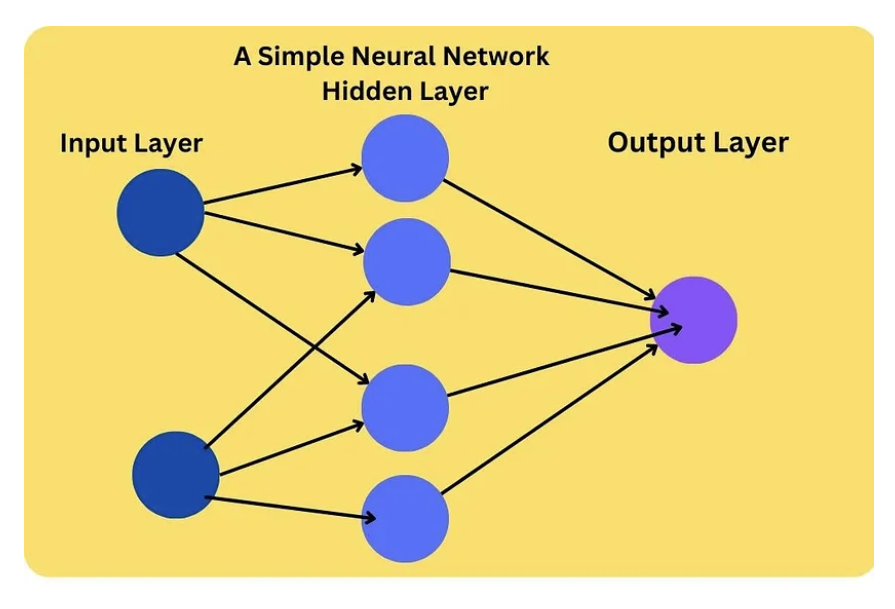
\includegraphics[scale=0.52]{./pics/ann.png}
  \caption[A simple Artificial Neural Network]{A simple Artificial Neural Network~\cite{ann}.}
  \label{fig:pi4}
\end{figure}

The three main layers in most ANNs are:

\begin{itemize}
  \item \textbf{Input Layer}: This layer receives the raw input data, which can be in various forms such as images, text, or numerical values.
  \item \textbf{Hidden Layers}: Located between the input and output layers, these layers are responsible for processing the input data through weighted connections and activation functions.
  \item \textbf{Output Layer}: The output layer produces the final results of the neural network’s processing, such as classifications or numerical predictions.
\end{itemize}

Training the neural network involves adjusting the weights of the connections to minimize the error in the output. Artificial neural networks have been successfully applied to a wide range of tasks, including Image Recognition, Natural Language Processing, Speech Recognition, Recommendation Systems, Financial Predictions, and many others. Their ability to learn and adapt from data makes them a powerful tool in Machine Learning and Artificial Intelligence.

\subsection{Multi-Layer Perceptron (MLP)}
Multilayer Perceptrons (MLPs) were initially inspired by the Perceptron, a supervised Machine Learning algorithm designed for binary classification. The original Perceptron was only capable of handling linearly separable data. To overcome this limitation, the Multilayer Perceptron was introduced, enabling the handling of both linearly and non-linearly separable data~\cite{mlp}.

An MLP is a type of neural network that belongs to the class of feed-forward neural networks. In these networks, the neurons in one layer are connected to the neurons in the subsequent layer in a forward manner, without any loops.

\begin{figure}[th]
  \centering
  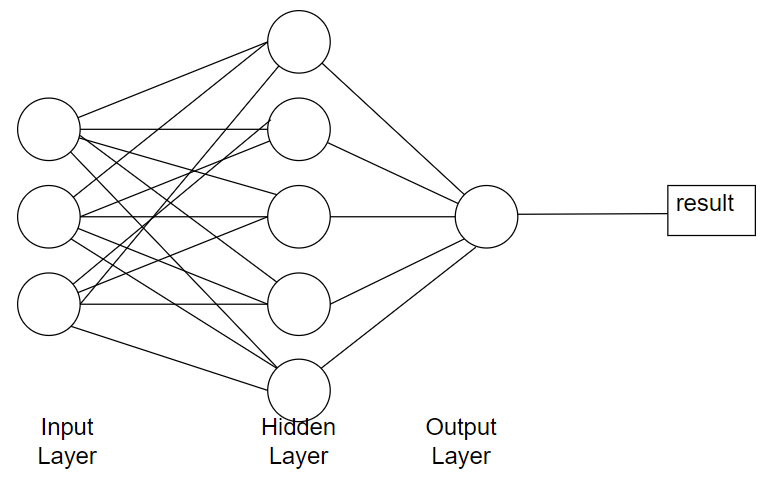
\includegraphics[scale=0.65]{./pics/mlp.png}
  \caption[Multilayer Perceptron]{Multilayer Perceptron~\cite{mlp}.}
  \label{fig:pi5}
\end{figure}

A Multilayer Perceptron (MLP) is a type of Artificial Neural Network (ANN) characterized by a layered architecture of interconnected neurons designed to process data through multiple stages. The fundamental structure of an MLP comprises an input layer, one or more hidden layers, an output layer, activation functions, and a set of weights and biases:

\begin{itemize}
  \item \textbf{Input Layer}: This is the initial layer that receives input data, which can be numerical values, images, or other types of structured data.
  \item \textbf{Hidden Layers}: Positioned between the input and output layers, these layers are responsible for processing the input data through complex computations. There is no fixed limit to the number of hidden layers, though MLPs usually feature a modest number to balance complexity and computational efficiency.
  \item \textbf{Output Layer}: The final layer that delivers the output results derived from the data processed throughout the network.
\end{itemize}

A defining feature of MLPs is the use of backpropagation, a supervised learning technique for training neural networks. Backpropagation involves adjusting the weights in the network by propagating the error from the output back through the network. This iterative process fine-tunes the network parameters, enhancing performance and minimizing errors.

Due to their straightforward design, MLPs typically require shorter training times to learn data representations and produce outputs. However, they often necessitate more powerful computing resources than standard computers, particularly devices equipped with Graphics Processing Units (GPUs), to handle the intensive computations involved.

MLPs have proven to be versatile and efficient tools in various applications, from image recognition and natural language processing to financial forecasting and beyond. Their ability to learn from data and improve over time underscores their importance in the realm of Machine Learning and Artificial Intelligence.

\subsection{Generative Adversarial Network (GAN)}
Generative Adversarial Networks (GANs)~\cite{goodfellow2014generative} have revolutionized the field of Artificial Intelligence, capturing widespread attention for their ability to generate and enhance data in innovative ways. They are pivotal in applications such as creating photorealistic images, transforming styles in artwork, and generating lifelike human faces. Introduced by Ian Goodfellow and his team in a groundbreaking 2014 NeurIPS paper, GANs~\cite{goodfellow2014generative} are specialized Machine Learning systems designed to mimic specific data distributions~\cite{gan}.

At the heart of a GAN~\cite{goodfellow2014generative} are two dynamically interacting neural networks: the Generator, which creates data, and the Discriminator, which evaluates the authenticity of the generated data. This dynamic interaction forms an "adversarial" training process, conceptualized as a competitive game. Here, the Generator strives to produce data so realistic that the Discriminator cannot reliably tell it apart from genuine data, achieving a 50\% deception rate.

A Generative Adversarial Network (GAN)~\cite{goodfellow2014generative} comprises two neural networks that engage in simultaneous adversarial training:

\begin{itemize}
  \item \textbf{Generator}: This network transforms random noise into coherent data outputs, such as images. Its objective is to generate data that closely resembles real-world data.
  \item \textbf{Discriminator}: This network evaluates both real data and data generated by the Generator, attempting to distinguish between the two. It outputs the likelihood that the provided data is real.
\end{itemize}

Throughout training, the Generator continuously improves its ability to create data that the Discriminator cannot distinguish from real data. Concurrently, the Discriminator enhances its skill in differentiating authentic data from the generated data. This adversarial "game" leads to the Generator producing progressively more realistic data over time.

Generative Adversarial Networks (GANs) employ loss functions to train both the generator and the discriminator, ensuring they both improve over time. The loss function helps adjust the weights of these models during training to enhance their performance. Both the generator and the discriminator utilize the binary cross-entropy loss, which can be expressed as~\cite{gan}:

\begin{equation}
  L(y, p) = - (y \log(p) + (1 - y) \log(1 - p))
\end{equation}

where:
\begin{itemize}
  \item \( L(y, p) \) is the loss value.
  \item \( y \) is the true label (either 0 or 1).
  \item \( p \) is the predicted probability of the sample belonging to class 1.
\end{itemize}

The discriminator objective is to correctly classify real samples as real and fake samples (generated by the generator) as fake. The loss for the discriminator is typically represented as~\cite{gan}:

\begin{equation}
  L_D = - \frac{1}{2} \mathbb{E}_{x \sim p_{data}(x)} [\log(D(x))] - \frac{1}{2} \mathbb{E}_{z \sim p_z(z)} [\log(1 - D(G(z)))]
\end{equation}

where:

\begin{equation}
  \mathbb{E}_{x \sim p_{data}(x)} [f(x)] \approx \frac{1}{N} \sum_{i=1}^{N} f(x_i)
\end{equation}

\begin{equation}
  \mathbb{E}_{z \sim p_z(z)} [f(z)] \approx \frac{1}{M} \sum_{i=1}^{M} f(z_i)
\end{equation}

In these equations:
\begin{itemize}
  \item \( x_i \) are samples from the real dataset.
  \item \( N \) is the number of samples from the real dataset.
  \item \( z_i \) are samples from the noise distribution.
  \item \( M \) is the number of samples from the noise distribution.
\end{itemize}

The first term on the right-hand side penalizes the discriminator for misclassifying real data, while the second term penalizes the discriminator for misclassifying the fake data produced by the generator.

The goal of the generator in a Generative Adversarial Network (GAN)~\cite{goodfellow2014generative} is to produce samples that the discriminator cannot distinguish from real data. The generator loss function is designed to penalize the generator when the discriminator correctly identifies its outputs as fake. Mathematically, the generator's loss can be expressed as~\cite{gan}:

\begin{equation}
  L_G = -\frac{1}{2} \mathbb{E}_{z \sim p_z(z)} \left[ \log(D(G(z))) \right]
\end{equation}

Here, \( z \) represents the noise input to the generator drawn from a prior distribution \( p_z(z) \), \( G(z) \) is the generated sample, and \( D(G(z)) \) is the discriminator probability that \( G(z) \) is a real sample.

The combined GAN~\cite{goodfellow2014generative} loss, also known as the minimax loss, encapsulates the adversarial nature of GAN~\cite{goodfellow2014generative} training. In this setup, the generator and discriminator engage in a two-player minimax game where the discriminator aims to maximize its ability to classify real and fake data correctly, while the generator strives to minimize the discriminator ability by generating realistic data. The combined loss is given by~\cite{gan}:

\begin{equation}
  L_{GAN} = \min_G \max_D (L_D + L_G)
\end{equation}

Here, \( L_D \) is the loss for the discriminator, and \( L_G \) is the loss for the generator.

Gradient penalty is a technique used to stabilize the training by penalizing the gradients if they become too steep. This can help in stabilizing the training and avoiding issues like mode collapse. The gradient penalty term is defined as~\cite{gan}:

\begin{equation}
  GP = \lambda \mathbb{E}_{\hat{x} \sim P_{\hat{x}}} \left[ \left( \| \nabla_{\hat{x}} D(\hat{x}) \|_2 - k \right)^2 \right]
\end{equation}

Where:
\begin{itemize}
  \item \(\mathbf{GP}\) represents the gradient penalty term.
  \item \(\mathbf{\lambda}\) is a hyperparameter that controls the strength of the penalty.
  \item The gradient component \(\nabla_{\hat{x}} D(\hat{x})\) is the gradient of the discriminator’s output with respect to its input \(\hat{x}\).
  \item \(\mathbf{P_{\hat{x}}}\) represents the distribution of interpolated samples between real and generated data.
  \item \(\mathbf{k}\) is a target norm for the gradient, often set to 1.
\end{itemize}

The purpose of introducing a gradient penalty is to enforce a constraint on the gradient of the discriminator output. This constraint ensures that the discriminator does not become overly confident, which can lead to sharp decision boundaries and unstable training. By keeping the gradient close to a target norm \(k\), typically set to 1, the gradient penalty helps maintain a smooth decision boundary.

The hyperparameter \(\lambda\) plays a crucial role in this process. A higher value of \(\lambda\) results in a stronger penalty for deviations from the target gradient norm, while a lower value of \(\lambda\) results in a weaker penalty. Proper tuning of \(\lambda\) is essential for the stability and performance of the GAN.

The interpolated samples \(\hat{x}\) are generated by taking convex combinations of real and generated samples. This interpolation helps in evaluating the gradient penalty across the data distribution, promoting better generalization and stability in the training process.

The discriminator loss with gradient penalty can be incorporated as follows:

\begin{equation}
  L_D = \mathbb{E}_{x \sim p_{\text{data}}(x)} \left[ \log(D(x)) \right] + \mathbb{E}_{z \sim p_z(z)} \left[ \log(1 - D(G(z))) \right] + GP
\end{equation}

This loss function consists of the usual GAN discriminator loss components for real and generated data, plus the gradient penalty term to regularize the discriminator behavior.


The discriminator loss with gradient penalty in GANs~\cite{goodfellow2014generative} integrates standard loss components for real and generated data, augmented by a gradient penalty term to regulate the discriminator behavior. By penalizing large gradients, this method promotes smoother behavior in the discriminator, contributing to a more stable training process for both the generator and the discriminator. The gradient penalty helps prevent sharp changes in the discriminator output, which can otherwise lead to instability and issues like mode collapse, where the generator produces limited and repetitive outputs.

\begin{figure}[th]
  \centering
  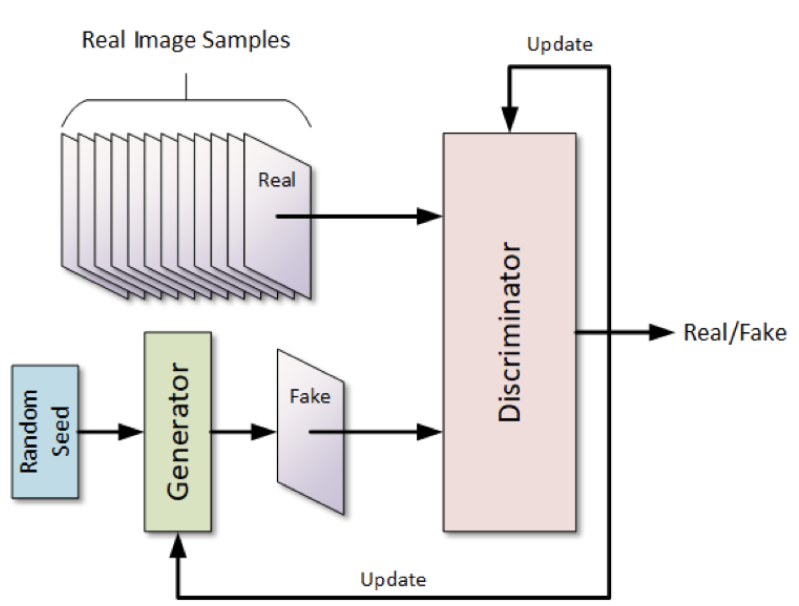
\includegraphics[scale=0.6]{./pics/gan.png}
  \caption[The Generative Adversarial Network Architecture]{The Generative Adversarial Network Architecture~\cite{gan-photo}.}
  \label{fig:pi6}
\end{figure}

GAN~\cite{goodfellow2014generative} are not only remarkable for their ability to create high-quality data, but also for their versatility across a range of complex tasks. Their unique adversarial training mechanism ensures that the generated data is continually refined, pushing the boundaries of what is possible in Machine Learning and Artificial Intelligence.

\subsection{Visual Transformer (ViTs)}

Originally designed for Natural Language Processing, the Transformer~\cite{vaswani2017attention} architecture has been successfully adapted to other domains~\cite{vit}.

\begin{figure}[th]
  \centering
  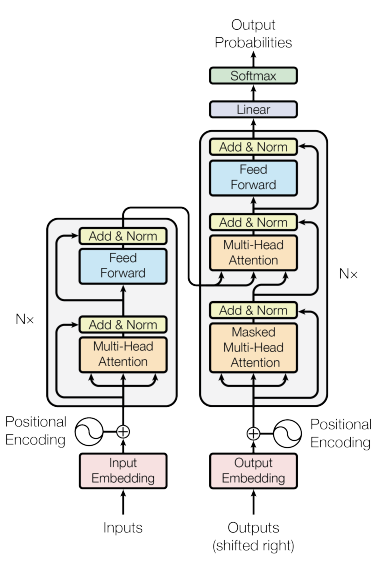
\includegraphics[scale=0.85]{./pics/transformer.png}
  \caption[The Transformer Architecture]{The Transformer Architecture~\cite{vaswani2017attention}.}
  \label{fig:pi7}
\end{figure}

A notable example is the Vision Transformer (ViT)~\cite{dosovitskiy2020}, which adapts the Transformer~\cite{vaswani2017attention} for Computer Vision tasks. In ViTs~\cite{dosovitskiy2020}, an image is divided into a sequence of patches, each linearly embedded and treated as input tokens for a stack of Transformer layers, collectively referred to as the Transformer Encoder.

The ViT has achieved state-of-the-art performance on various image classification benchmarks, showcasing the Transformer~\cite{vaswani2017attention} architecture's versatility and effectiveness across different domains.

Visual Transformer (ViT)~\cite{dosovitskiy2020} is a Deep Learning architecture that leverages the self-attention mechanism of Transformers~\cite{vaswani2017attention} to process and understand visual data such as images~\cite{vit}.

By dividing an input image into smaller patches, ViT~\cite{dosovitskiy2020} allows each patch to attend to others, leading to state-of-the-art performance in various computer vision tasks

The usual workflow of Visual Transformers~\cite{dosovitskiy2020} in Image Classification task include~\cite{vit}:

\begin{enumerate}
  \item Decomposing the Image into Patches
        \begin{itemize}
          \item \textbf{Input Image}: Consider an input image with dimensions \( H \times W \times N \), where \( H \) is the height, \( W \) is the width, and \( N \) represents the number of channels (such as 3 for RGB images).
          \item \textbf{Patch Flattening}: The image is divided into smaller patches, each of size \( 16 \times 16 \) pixels. For an RGB image, this results in each patch being flattened into a vector of 768 elements (since \( 16 \times 16 \times 3 = 768 \)). This transformation converts the spatial information of the image patches into a form suitable for further processing by the Vision Transformer.
        \end{itemize}

  \item Patch Embedding
        \begin{itemize}
          \item \textbf{Linear Transformation}: Each flattened patch undergoes a trainable linear transformation that maps it into a \( D \)-dimensional embedding space. This operation, which is akin to a fully connected layer, enriches the representation of each patch, making it more suitable for subsequent processing by the transformer.
          \item \textbf{Spatial Information Encoding}: Since the transformer architecture does not inherently preserve the spatial arrangement of patches, additional spatial information is incorporated into the patch embeddings. This is achieved by adding positional encodings, which can be either fixed or learned parameters, to the embedded patches. These encodings ensure that the model retains information about the position of each patch within the original image.
        \end{itemize}

  \item Visual Transformer Encoder
        \begin{itemize}
          \item \textbf{Self-Attention Mechanism}: At the heart of the transformer model lies the self-attention mechanism, which efficiently evaluates the relevance of different patches in relation to each other for a specific task. This mechanism determines the amount of focus each part of the image should receive when encoding a particular patch, enhancing the model's ability to understand complex relationships within the image.
          \item \textbf{Multi-head Attention}: The encoder employs multi-head attention, running several self-attention mechanisms in parallel. This approach allows the model to simultaneously capture diverse aspects and patterns in the image, enriching the representation of each patch with a variety of contextual information.
          \item \textbf{Feed-forward Network}: Following the attention computation, each patch's representation is processed through a feed-forward neural network (FFNN). This network is applied identically and independently to each position, further refining the encoded information and enabling the model to learn intricate features.
          \item \textbf{Residual Connections and Normalization}: To ensure a stable training process and facilitate the accumulation of knowledge from each layer, the transformer encoder incorporates residual connections around each sub-layer. These are followed by layer normalization, which helps maintain consistent gradients and improves the overall training dynamics, ensuring that each layer effectively builds upon the previous ones.
        \end{itemize}

  \item Creating the Output
        \begin{itemize}
          \item \textbf{CLS Token}: To adapt transformer architecture for image classification, a dedicated classification token (CLS) is prefixed to the sequence of embedded patches. This token encapsulates comprehensive information aggregated from the entire image after undergoing transformation through the encoder. Utilized by a classifier, typically a straightforward linear layer, it facilitates accurate prediction of the image's class by leveraging enriched contextual understanding encoded within the transformer model.
        \end{itemize}

  \item Training
        \begin{itemize}
          \item \textbf{Optimizing Model Parameters}: During training, the transformer model is fine-tuned end-to-end using an appropriate loss function, commonly cross-entropy for classification tasks. This function calculates the discrepancy between predicted and actual class labels, guiding the optimization of parameters across the linear projection, transformer encoder, and classifier. The objective is to systematically minimize this loss on a training dataset, ensuring the model effectively learns to classify images with high accuracy.
        \end{itemize}
\end{enumerate}

\begin{figure}[th]
  \centering
  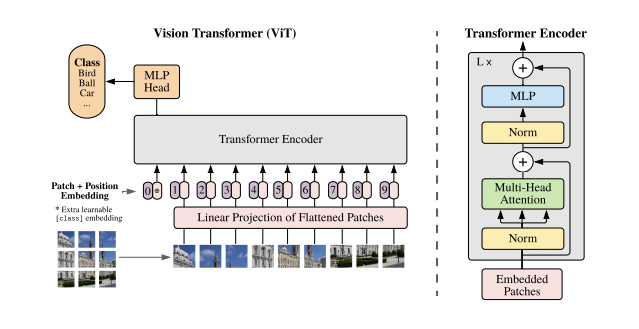
\includegraphics[scale=0.8]{./pics/vit.png}
  \caption[The Visual Transformer Neural Architecture]{The Visual Transformer Neural Architecture~\cite{vaswani2017attention, dosovitskiy2020}.}
  \label{fig:p8}
\end{figure}

The transformation at each layer can be defined as~\cite{Comajoan_Cara_2024}:

\begin{equation}
  Z = X + \text{LayerNorm}(\text{MHA}(X, X, X))
\end{equation}

\begin{equation}
  X' = Z + \text{LayerNorm}(\text{MLP}(Z))
\end{equation}

where \( X \in \mathbb{R}^{N \times D} \) is a Transformer layer matrix input and  \( X' \in \mathbb{R}^{N \times D} \) is the output.

The attention mechanism is a vital component of the Transformer architecture, enabling the model to focus on specific parts of the input sequence when generating each output element. Given a query matrix \( Q \in \mathbb{R}^{N \times D_k} \), a key matrix \( K \in \mathbb{R}^{M \times D_k} \), and a value matrix \( V \in \mathbb{R}^{M \times D_v} \), the attention function is defined as~\cite{Comajoan_Cara_2024}:

\begin{equation}
  \text{Attention}(Q, K, V) = \text{softmax}\left(\frac{QK^T}{\sqrt{D_k}}\right) V
\end{equation}

where \( D_k \) is the dimension of the keys, used as a scaling factor to prevent the dot products from becoming excessively large.

Self-attention is a specialized form of attention where the query, key, and value matrices are all derived from the same input matrix \( X \). Within the Transformer, self-attention permits each position in the input sequence to attend to all other positions in the preceding layer.

Multi-head attention augments the attention mechanism, enabling the model to concurrently attend to information from diverse representation subspaces at different positions. Rather than executing a single attention function, multi-head attention projects the queries, keys, and values \( h \) times using different learned linear projections. These projections are processed in parallel, their results concatenated, and the concatenated output is then linearly projected once more. Mathematically, multi-head attention is expressed as~\cite{Comajoan_Cara_2024}:

\begin{equation}
  \text{MHA}(Q, K, V) = \text{Concat}(\text{head}_1, \ldots, \text{head}_h) W^O
\end{equation}

\begin{equation}
  \text{head}_i = \text{Attention}(Q W_i^Q, K W_i^K, V W_i^V)
\end{equation}

Here, \( W_i^Q \in \mathbb{R}^{D_x \times D_k} \), \( W_i^K \in \mathbb{R}^{D_x \times D_k} \), \( W_i^V \in \mathbb{R}^{D_x \times D_v} \), and \( W^O \in \mathbb{R}^{h D_v \times D_x} \) are learnable parameter matrices.


\subsection{Learning Rate Schedulers}
When training deep networks, it's beneficial to gradually reduce the learning rate as the training progresses. This concept stems from the idea that a high learning rate imparts high kinetic energy to the model, causing its parameter vector to oscillate chaotically. Consequently, the model struggles to stabilize within the deeper and narrower valleys of the loss function, which represent local minima. Conversely, if the learning rate is too low, the system exhibits low kinetic energy, leading it to settle into the shallower and narrower valleys of the loss function, often getting stuck in suboptimal minima.

In essence, starting with a higher learning rate helps the model explore the loss landscape broadly, avoiding premature convergence. As training advances, lowering the learning rate allows the model to fine-tune its parameters and settle into more optimal solutions, thus achieving better performance. This dynamic adjustment helps in navigating the complex loss surfaces typical in deep learning, striking a balance between exploration and exploitation~\cite{learningrate}.

Examples of Learning Rate Scheduling~\cite{learningrate2}:

\begin{itemize}
  \item ExponentialLR: Adjusts the learning rate by dividing it by a factor each epoch or evaluation period.
  \item CyclicLR: Oscillates the learning rate cyclically between specified minimum and maximum values.
  \item StepLR: Decreases the learning rate by multiplying it with a decay factor every fixed number of epochs or evaluation periods.
  \item MultiStepLR: Reduces the learning rate by a factor when the training reaches predefined milestones.
  \item ReduceLROnPlateau: Dynamically reduces the learning rate if a monitored metric fails to improve for a certain number of evaluations.
  \item CosineAnnealingLR: Starts with a high learning rate and smoothly decreases it following a cosine curve, periodically restarting the cycle.
\end{itemize}

\subsection{Weight Decay}
Weight decay, also known as L2 regularization, is an essential technique in deep learning to enhance model performance. By penalizing large weights, it offers several key benefits~\cite{weightdecay}:

\begin{itemize}
  \item \textbf{Mitigates Overfitting:} Large weights often cause a model to memorize training data, hindering its ability to generalize to new examples. Weight decay discourages large weights, promoting the learning of smaller, more generalizable weights that capture the fundamental patterns in the data.

  \item \textbf{Enhances Model Stability:} Large weights can destabilize training and increase sensitivity to data noise. Weight decay stabilizes the training process by keeping weights manageable, thus enhancing the model's robustness and reducing overfitting.

  \item \textbf{Encourages Feature Sharing:} By promoting similar weights across different neurons, weight decay fosters feature sharing. This leads to a more efficient network where multiple neurons can utilize the same features, often resulting in fewer required parameters.

  \item \textbf{Boosts Generalization in Overparameterized Models:} Modern deep learning models often contain more parameters than training data, a scenario known as overparameterization. Weight decay helps manage the complexity of such models, improving their ability to generalize.
\end{itemize}

Weight decay adds a penalty to the loss function, proportional to the sum of the squared weights. This penalty encourages the model to prefer smaller weights during training. Implementation of weight decay typically follows one of two approaches:

\begin{itemize}
  \item \textbf{L2 Regularization:} Adds a term to the loss function proportional to the sum of the squared weights.
  \item \textbf{Optimizer-based Weight Decay:} Alters the optimizer's update rule to include a decay factor that incrementally reduces the weights.
\end{itemize}

Choosing the right weight decay parameter involves balancing overfitting prevention with performance optimization. The optimal value varies based on model size, complexity, training data, and learning rate. Techniques such as grid search, hyperparameter optimization, and cross-validation are useful for identifying the best weight decay value.

\subsection{Cross Validation}
Cross-Validation (CV) is a cornerstone of evaluating learning models which provides the possibility to approximate model performance on unseen data not used while training. When training a model, the dataset is divided into two primary subsets: training and testing. The training set encompasses all the examples from which the model learns, while the testing set emulates real-world scenarios where the model performance is assessed~\cite{crossvalidation}.

Validating a learning model before deploying it in production involves ensuring it can make accurate predictions on data it has never encountered. This unseen data represents any type of information that the model hasn't been trained on. Ideally, during testing, this data flows directly into the model across numerous iterations. However, in practice, access to genuinely new data is often restricted or unavailable in a fresh environment.

A common approach is the 80-20 rule, where 80\% of the data is used for training and 20\% for testing. Despite its popularity, this method is prone to creating a seemingly perfect split that might artificially inflate model accuracy, while failing to replicate the same performance in real-world scenarios. The accuracy achieved in such cases can often be attributed to mere chance. It is worth noting that the 80-20 split is not a hard and fast rule; other ratios like 70-30 or 75-25 are frequently used as well.

Tuning model hyperparameters is another crucial step in optimizing an algorithm to uncover the hidden patterns within a dataset. However, performing this tuning on a simple training-testing split is generally discouraged. Model performance is highly sensitive to hyperparameters, and adjusting them based on a fixed data split can lead to overfitting, reducing the model generalizability~\cite{crossvalidation}.

To avoid overfitting during hyperparameter tuning, some suggest dividing the dataset into three parts: training, validation, and testing, for example, using 70\% for training, 20\% for validation, and 10\% for testing. Yet, with small datasets, maximizing the data for training is often necessary. Moreover, such splits can introduce bias if important examples are disproportionately allocated to the training or validation sets. Cross-validation (CV) is a valuable technique to mitigate these issues by ensuring a more balanced evaluation.

The process of splitting data for training and testing can be fraught with difficulties. The testing set may not share similar properties with the training set, causing instability. Even though random sampling theoretically gives each sample an equal chance of being included in the testing set, a single split might still result in instability when the experiment is repeated with a different division.


\subsection{Random Search}
Random Search is a hyperparameter optimization technique in machine learning that samples a defined number of hyperparameter combinations from specified distributions at random. These distributions represent sets or ranges of possible parameter values~\cite{randomsearch}.

This method efficiently navigates a subset of the hyperparameter space, making it faster and more resource-efficient compared to exhaustive techniques like grid search.

Although Random Search may not guarantee the discovery of the absolute optimal hyperparameters, it is highly effective at identifying good configurations, particularly in scenarios involving large or complex parameter spaces.

\section{Ordinary Differential Equations (ODE)}
TODO

\subsection{Runge-Kutta Methods}
TODO

\subsection{ODE Interpretation of Transformer Layers}
TODO

\section{Quantum Computing}
TODO

\subsection{Quantum Gates}
TODO

\subsection{Quantum Circuits}
TODO

\subsection{Quantum Machine Learning}
TODO

\subsection{Variational Quantum Circuits (VQC)}
TODO

\subsection{Quantum Runge-Kutta Method}
TODO

\subsection{Quantum Transformer}
TODO

\chapter{Proposed Solution}\pagestyle{fancy}

\chapter{Experiments}\pagestyle{fancy}

\chapter{Conclusions and Future Work}\pagestyle{fancy}

\chapter{Bibliography}\pagestyle{fancy}

\bibliographystyle{unsrt}

\begingroup
\def\chapter*#1{}
\bibliography{bibliography}
\endgroup

\end{document}
